\chapter{Asymptotic Safety of Gravity-Matter Systems}\label{chap:Matter} 
The calculation in $h^{\mathrm{TT}}$ approximation in the last chapter already allowed us to investigate the characteristic fixed point structure of the Einstein-Hilbert truncation. Nevertheless, in this part of the thesis, where the impact of minimally coupled matter fields is investigated, we want to work with the full result, including also the vector and scalar modes arising after the York decomposition (\ref{eqn:York}) of the fluctuation field. This also means, that we have to take care of additional gauge fixing and ghost terms, given by 
\begin{align}
\mathcal{S}_{\mathrm{gf}} &= \frac{1}{2\alpha} \int_x \sqrt{\bar{g}} \  \bar{g}^{\mu\nu} F_{\mu}F_{\nu}	\nonumber\\
\phantom{.} \\
\mathcal{S}_{\mathrm{gh}} &= \int_x \sqrt{\bar{g}} \  \bar{g}^{\mu\mu'} \bar{g}^{\nu\nu'}\bar{c}_{\mu'} \mathcal{M}_{\mu\nu}  c_{\nu'} \nonumber
\end{align}
with the Faddeev-Popov operator $\mathcal{M}_{\mu\nu}(\bar{g},h)$ for the gauge fixing $F_{\mu}(\bar{g},h)$. 
\begin{align}
	F_{\mu} &= \bar{\nabla}^{\nu}h_{\mu\nu} - \frac{1+\beta}{4}\bar{\nabla}_{\mu}h^{\nu}_{\phantom{\nu}\nu} \nonumber \\
	\phantom{.} \\
	\mathcal{M}_{\mu\nu} &= \bar{\nabla}^{\rho}(g_{\mu\nu}\nabla_{\rho} + g_{\rho\nu}\nabla_{\mu}) - \bar{\nabla}_{\mu}\nabla_{\nu}, \nonumber
\end{align}


%TODO: Explain which formulas we are using and introduce gauge fixing etc. Reference to Pawlowski script..
 
The inclusion of matter in this theory setting is in principle straightforward. We extend our truncation (\ref{eqn:QGflow}) by including an additional matter term: 
\begin{align}
	\Gammak = \Gamma_{\text{EH}} + \mathcal{S}_{\text{gf}}+ \mathcal{S}_{\text{gh}}+ \Gamma_{\text{matter}},
\end{align}
where $\Gamma_{\mathrm{matter}}$ consists of scalar, fermion and gauge field contributions, denoted with $\mathcal{S}_S, \mathcal{S}_D$ and $\mathcal{S}_V$ respectively:
\begin{align}
	\Gamma_{\text{matter}} = \mathcal{S}_S + \mathcal{S}_D + \mathcal{S}_V.
\end{align}
The different actions will be specified later on, every matter type will be treated separately. For conventions regarding the choice of the respective regulators and the general structure of this calculation, we are following \cite{DonaEichhornPercacci2013}. \\
In this truncation we have two essential couplings, $G$ and $\Lambda$ and five inessential\footnote{Inessential in this sense means, that they can be eliminated by field rescalings.} wave function renormalizations $Z_{\Psi}$ with $\Psi = (h,c,S,D,V)$. As before, the wave function renormalizations $Z_{\Psi}$ do not enter the beta functions for $G$ and $\Lambda$ directly, but are still present in a non-trivial way via the anomalous dimension $\eta_{\Psi}$, defined as
\begin{align}
	\eta_{\Psi} = -\partial_t \ln Z_{\Psi}.
\end{align}
For the scalar and gauge field regulators we choose
\begin{align}
	R_{k,\sfrac{S}{V}}(z) = Z_{\sfrac{S}{V}} \cdot \mathbbm{1}_{\sfrac{S}{V}} \cdot \tilde{\Delta}\cdot r_k\left(\frac{\tilde{\Delta}}{k^2}\right),
	\label{eqn:Rk_matter}
\end{align}
where $\tilde{\Delta}= -\nabla^2 + \mathbf{E}_{\Psi}$ is a modified Laplacian\footnote{A more detailed discussion on how these modified Laplacians effect the values of the heat-kernel coef-\\ \phantom{........}ficients is presented in appendix \ref{chap:AppA}.}, occurring as kinetic operator in the different matter field actions. The regulator choice for the Dirac fermions is slightly different, details are discussed in the respective subsection. Nevertheless, we already present the values of $\mathbf{E}_{\Psi}$ for all three kinetic operators:
\begin{align}
	\mathbf{E}_{\Psi} =  \left\{\begin{array}{ll}{0} & {\text { for } \Psi = S} \\[5pt] {\frac{\mathcal{R}}{4}} & {\text { for } \Psi = D}\\[5pt]  {R^{\mu}_{\phantom{\mu}\nu}} & {\text { for } \Psi = V.}\end{array}\right.
\end{align}
The Litim-type shape function $r_k$ is in this case the same as the one defined in equation (\ref{eqn:Litim}), now as a function of the modified Laplacian $\tilde{\Delta}$.
%TODO: Some words on fermions ...
\section{Matter Contributions in Background Field Approximation}
After having introduced the setup for the following calculation, we are now able to determine the different contributions from the matter fields step by step, by evaluating the functional traces ocurring on the r.\,h.\,s. of the flow equation separately. For the matter configuration in our setting the flow equation reads
\begin{equation}
\begin{aligned}
 \partial_t\Gamma_{k} =\frac{1}{2} \operatorname{Tr}&\left[\left(\Gamma^{(2)}+R_{k}\right)^{-1} \partial_t R_{k}\right]_{h h} - \operatorname{Tr}\left[\left(\Gamma^{(2)}+R_{k}\right)^{-1} \partial_t R_{k}\right]_{\bar{c}c}\\[10pt]
 + \frac{1}{2}\operatorname{Tr}&\left[\left(\Gamma^{(2)}+R_{k}\right)^{-1} \partial_t R_{k}\right]_{\phi\phi}  -\operatorname{Tr}\left[\left(\Gamma^{(2)}+R_{k}\right)^{-1}\partial_t R_{k}\right]_{\bar{\psi} \psi} \\[10pt]
 +\frac{1}{2} \operatorname{Tr}&\left[\left(\Gamma^{(2)}+R_{k}\right)^{-1}\partial_t R_{k}\right]_{AA}.\end{aligned}
\label{eqn:matter_flow}
\end{equation}
%TODO: Explain signs and prefactors
In figure (\ref{fig:matter_calc}), a digrammatical representation of the flow equation (\ref{eqn:matter_flow}) is depicted.
\begin{figure}[t]
	\centering
	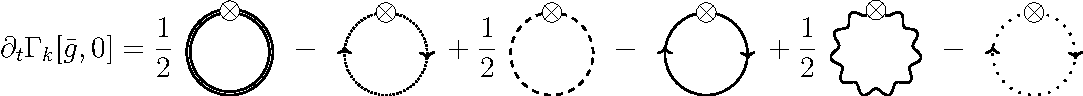
\includegraphics[width=0.95\textwidth]{figs/TikZ/matter_corrections}
\caption[Flow equation for the average effective action $\Gamma_k$ including different matter contributions in diagrammatic representation.]{Flow equation (\ref{eqn:matter_flow}) for the average effective action $\Gamma_k$ including different matter contributions in diagrammatic representation. The double, dotted,dashed, solid and  wiggly lines correspond to the graviton, ghost, scalar, fermion and gauge field  propagators, respectively. The crossed circles denote the insertion of the respective regulator.}
	\label{fig:matter_calc}
	\hrulefill
\end{figure}

\subsection{Scalar fields}
The action for $N_S$ scalar fields, minimally coupled to gravity reads
\begin{align}
	\mathcal{S}_S &= \frac{Z_{S}}{2}\int_x \sqrt{g} \ g^{\mu\nu} \ \sum\limits_{i=1}^{N_{\text{S}}} \partial_{\mu}\phi^{i}\partial_{\nu}\phi^{i} \nonumber \\
&=  \frac{Z_{S}}{2}\int_x \sqrt{\bar{g}} \ \bar{g}^{\mu\nu} \ \sum\limits_{i=1}^{N_{\text{S}}} \partial_{\mu}\phi^{i}\partial_{\nu}\phi^{i} + \mathcal{O}(h) \\
&= \frac{Z_{S}}{2}\int_x \sqrt{\bar{g}} \ \ \sum\limits_{i=1}^{N_{\text{S}}} \phi^{i}\left(-\bar{\nabla}^2\right)\phi^{i} + \mathcal{O}(h). \nonumber
\end{align}
For our computation, we expand the action on some background $\bar{g}_{\mu\nu}$ and drop all contributions of $\mathcal{O}(h)$. In the last step, we use integration by parts and assume vanishing boundary terms. Since $\mathbf{E} =0$ for scalars, we use the initial definition of the Laplacian $\bar{\Delta} = -\bar{\nabla}^2$ for further calculations. These simple manipulations directly allow us to read off the corresponding two-point function
\begin{align}
	\Gamma^{(2)}_{\phi\phi} = \frac{\delta^2 \mathcal{S}_S}{\delta\phi^{i}\ \delta\phi^{j}} = Z_S \cdot\bar{\Delta}\cdot\mathbbm{1}_S + \mathcal{O}(h),
\end{align}
where $\mathbbm{1}_S$ has to be understood as the identity in field space. Using the regulator defined in (\ref{eqn:Rk_matter}), we find the regularized two-point-function as
\begin{align}
	\Gamma^{(2)}_{k, \phi\phi} = \left[\Gamma^{(2)}_{\phi\phi}+ R_{k, S}\right]  = Z_S \cdot\bar{\Delta}\cdot\mathbbm{1}_S\left(1 + r_k\left(\frac{\bar{\Delta}}{k^2}\right)\right).
\end{align}
This expression is already diagonal in field space, meaning we are directly able to invert it to obtain the propagator. Together with the scale derivative of the regulator
\begin{align}
	\partial_t R_{k, S} = Z_S\cdot\mathbbm{1}_S\cdot\bar{\Delta}\left(\partial_t r_k - \eta_S r_k\right),
\end{align}
we can start to evaluate the r.\,h.\,s. of the flow equation:
\begin{align}
	\frac{1}{2}\tr{\left(\Gamma^{(2)}_{k, \phi\phi}\right)^{-1}\partial_t R_{k,S}} &= \frac{1}{2}\tr{\frac{Z_S\bar{\Delta}\left(\partial_t r_k - \eta_s r_k\right)}{Z_S \bar{\Delta}\left(1 + r_k\right)}\mathbbm{1}_S} \nonumber\\
	\phantom{.} \\
	&=   \frac{N_S}{2}\tr{\frac{\bar{\Delta}\left(\partial_t r_k - \eta_s r_k\right)}{\bar{\Delta}\left(1 + r_k\right)}}. \nonumber
\end{align}
Here, we already performed the trace operation on the internal indices, leading to an overall factor of $N_S$. The functional trace is again evaluated using heat-kernel techniques.
\begin{equation}
\begin{aligned}
	\frac{N_S}{2}\tr{\frac{\bar{\Delta}\left(\partial_t r_k - \eta_s r_k\right)}{\bar{\Delta}\left(1 + r_k\right)}} &= \frac{N_S}{2}\frac{1}{(4\pi^2)}\left[\int_x\sqrt{\bar{g}} \  \Phi_2^1(0) + \frac{1}{6}\int_x\sqrt{\bar{g}} \ \bar{\mathcal{R}}\ \Phi_1^1(0) \right]\\[10pt]
	&= 	\frac{N_S}{2}\frac{1}{(4\pi)^2}\int_x\sqrt{\bar{g}}\left[\left(1-\frac{\eta_S}{6}\right) + \frac{\bar{\mathcal{R}}}{3}\left(1-\frac{\eta_S}{6}\right)\right].
\end{aligned}
\end{equation}
\subsection{Fermionic  fields}
For the fermionic contribution, we  proceed slightly different. First, we present the action for $N_D$ minimally coupled Dirac fermions:
\begin{equation}
	\begin{aligned}
		\mathcal{S}_D &= iZ_D\int_x \sqrt{g} \ \sum\limits_{i=1}^{N_D}\bar{\psi}^{i}\slashed{\nabla}\psi^{i} \\[10pt]
		&=  iZ_D\int_x \sqrt{\bar{g}} \ \sum\limits_{i=1}^{N_D}\bar{\psi}^{i}\bar{\slashed{\nabla}}\psi^{i} + \mathcal{O}(h).
	\end{aligned}
\end{equation}
The Dirac operator $\slashed{\nabla}$ satisfies $-\slashed{\nabla}^2 = -\nabla^2 + \frac{\bar{\mathcal{R}}}{4} := \Delta_{\left(\sfrac{1}{2}\right)}$.
The notation for the conjugated field $\bar{\psi} = \psi^{\dagger}\mathfrak{h}$\footnote{The spin metric $\mathfrak{h}$ satisfies $\abs{\operatorname{det} \mathfrak{h}} = 1$ and $\mathfrak{h}^{-1} = -\mathfrak{h}$.} should not be confused with the bar referring to the background field. As usual, the slashed notation implies contraction with gamma matrices\footnote{In the discussion of Dirac fermions, the gamma matrices $\left\{\gamma^0, \gamma^1, \gamma^2, \gamma^3\right\}$ are a set of complex valued matrices, that constitute an irreducible representation of the Clifford algebra, defined by the anticommutation relation $\left\{\gamma_{\mu}, \gamma_{\nu}\right\}= 2g_{\mu\nu} \mathbbm{1}_{d_{\gamma}\times d_{\gamma}}$, with $d_{\gamma} = 2^{\left[\sfrac{d}{2}\right]}$. A more formal treatment of fermions in curved spacetimes is presented in \cite{LippoldtPHD}.}, i.\,e. $\slashed{\nabla} = \gamma^{\mu}\nabla_{\mu}$.  \\
In principle, this allows us to read off the fermion two-point function
\begin{align}
	\Gamma^{(2)}_{\bar{\psi}\psi} = \frac{\delta^2 \mathcal{S}_D}{\delta \psi^{i}\ \delta \bar{\psi}^{j}} = iZ_D\cdot\slashed{\nabla}\cdot\mathbbm{1}_D + \mathcal{O}(h).
\end{align}
In general one chooses the regulator, such that the symmetries of the kinetic term are conserved. As before, the general form of such a regulator is given by
\begin{align}
	R_{k,D} = Z_D\cdot\tilde{\Delta}\cdot\mathbbm{1}_D\cdot r_{k, D}\left(\frac{\tilde{\Delta}}{k^2}\right).
\end{align} 
When computing fermion propagators in other theory settings, it follows quite naturally to consider the Dirac dispersion as the "square root" of the scalar Klein-Gordon dispersion. For a more detailed discussion of this idea in the context of Fermi-Bose mixtures, we refer to chapter 2 of \cite{PawlowskiNPgaugeLecture} or in the context of gravity-matter systems in quantum gravity to the appendix of \cite{BritoHamadaPereiraYamada2019}. \\
This assumption allows us to express $r_k$ for the fermions as a function of the scalar shape function:
\begin{align}
\left[1+r_{k,D}\right]^2 = 1+r_{k,S} \qquad \longrightarrow \qquad r_{k, D} = \sqrt{1+r_{k,S}} - 1
\end{align}
In total, this yields the final expression for regularized two-point function for the fermions:
\begin{align}
	\Gamma^{(2)}_{\bar{\psi}\psi, k} = 
\end{align}
%TODO: To do..
\subsection{Gauge fields}  
The structure of the gauge field contribution is more complex than for the other fields. This is due to the fact, that we have to employ a gauge fixing procedure w.\,r.\,t. the background field $\bar{g}_{\mu\nu}$. This ensures gauge invariance w.\,r.\,t. background gauge transformations. The action for $N_V$ gauge fields, minimally coupled to gravity reads
\begin{equation}
\begin{aligned}
\mathcal{S}_{V} &= \frac{Z_{\text{V}}}{4}\int_x \sqrt{g} \ \sum\limits_{i=1}^{N_{\text{V}}} g^{\mu\nu}g^{\kappa\lambda}F^{i}_{\mu\kappa}F^{i}_{\nu\lambda}  
		+ \frac{Z_{\text{V}}}{2\xi}\int_x \sqrt{\bar{g}} \ \sum\limits_{i=1}^{N_{\text{V}}} \left(\bar{g}^{\mu\nu}\bar{\nabla}_{\mu}A_{\nu}^{i}\right)^2\\
		&+\int_x \sqrt{\bar{g}} \ \sum\limits_{i=1}^{N_{\text{V}}} \bar{C}_i(-\bar{\nabla}^2)C_i, 
\end{aligned}
\end{equation}
where the second term is the gauge fixing term with gauge parameter $\xi$ and the third term is the Abelian ghost term. Since the two-point function is obtained from a functional derivative w.\,r.\,t. the fields $A^{i}$, we have to evaluate the ghost-term separately. We start by manipulating the first term:
\begin{equation}
\begin{aligned}
\frac{Z_V}{4}\int_x \sqrt{g} \ \sum\limits_{i=1}^{N_{\text{V}}} g^{\mu\nu}g^{\kappa\lambda}F^{i}_{\mu\kappa}F^{i}_{\nu\lambda} =  \frac{Z_{V}}{4} &\int_x \sqrt{\bar{g}} \ \sum\limits_{i=1}^{N_{\text{V}}} \bar{g}^{\mu\nu}\bar{g}^{\kappa\lambda}\bar{F}^{i}_{\mu\kappa}\bar{F}^{i}_{\nu\lambda} + \mathcal{O}(h) \\[5pt]
\overset{(\mathrm{\ref{eqn:FF2}})}{=} \frac{Z_{V}}{2} &\int_x \sqrt{\bar{g}} \ \sum\limits_{i=1}^{N_{\text{V}}} A_{\lambda}^{i}\left[ \bar{\nabla}^{\mu}\bar{\nabla}^{\lambda} - \bar{g}^{\mu\lambda}\bar{\nabla}^2\right]A_{\mu}^{i} + \mathcal{O}(h).
\end{aligned}
\end{equation}
%TODO: Alignment..
The steps we skipped can be found in appendix \ref{chap:AppB}. For the gauge fixing term we find:
\begin{equation}
\begin{aligned}
\frac{Z_{\text{V}}}{2\xi}\int_x \sqrt{\bar{g}} \ \sum\limits_{i=1}^{N_{\text{V}}} \left(\bar{g}^{\mu\nu}\bar{\nabla}_{\mu}A_{\nu}^{i}\right)^2 
	&= \frac{Z_{\text{V}}}{2\xi}\int_x \sqrt{\bar{g}} \ \sum\limits_{i=1}^{N_{\text{V}}} \bar{g}^{\mu\nu}\bar{\nabla}_{\mu}A_{\nu}^{i}g^{\kappa\lambda}\bar{\nabla}_{\kappa}A_{\lambda}^{i} \\[5pt]
	&= \frac{Z_{\text{V}}}{2\xi}\int_x \sqrt{\bar{g}} \ \sum\limits_{i=1}^{N_{\text{V}}} A_{\lambda}^{i}\left[-\bar{\nabla}^{\lambda}\bar{\nabla}^{\mu}\right]A_{\mu}^{i}. 
\end{aligned}	
\end{equation}
In the last step, we integrated by parts and assumed vanishing boundary terms.\\
 This allows us to write 
\begin{equation}
\mathcal{S}_V = \frac{Z_{V}}{2} \int_x \sqrt{\bar{g}} \ \sum\limits_{i=1}^{N_{\text{V}}} A_{\lambda}^{i}\left[ - \bar{g}^{\mu\lambda}\bar{\nabla}^2 +  \bar{\nabla}^{\mu}\bar{\nabla}^{\lambda} - \frac{1}{\xi} \bar{\nabla}^{\lambda}\bar{\nabla}^{\mu}\right]A_{\mu}^{i} \ + \ \text{ghost term}
\end{equation}
In Feynman gauge, where we set $\xi \equiv 1$, this simplifies to
\begin{equation}
\begin{aligned}
\mathcal{S}_V &= \frac{Z_{V}}{2} \int_x \sqrt{\bar{g}} \ \sum\limits_{i=1}^{N_{\text{V}}} A_{\lambda}^{i}\left[ - \bar{g}^{\mu\lambda}\bar{\nabla}^2 +  \left[\bar{\nabla}^{\mu}, \bar{\nabla}^{\lambda}\right]\right]A_{\mu}^{i} \ + \ \text{ghost term} \\
&\overset{(\mathrm{\ref{eqn:RiemannB}})}{=} \frac{Z_{V}}{2} \int_x \sqrt{\bar{g}} \ \sum\limits_{i=1}^{N_{\text{V}}} A_{\lambda}^{i}\left[ - \bar{g}^{\mu\lambda}\bar{\nabla}^2 +  \bar{R}^{\mu\lambda}\right]A_{\mu}^{i} \ + \ \text{ghost term}
\end{aligned}
\end{equation}
%TODO: Aligning equation

In this form, we are again directly able to read off the two-point-function:
\begin{equation}
	\Gamma^{(2)}_{AA} = \frac{\delta^2 \mathcal{S}_V}{\delta A^{i}\ \delta A^{j}} = Z_V\underbrace{\left[ - \bar{g}^{\mu\lambda}\bar{\nabla}^2 +  \bar{R}^{\mu\lambda}\right]}_{=: \  \bar{\Delta}^{\mu\nu}_{(1)}}\mathbbm{1}_V + \mathcal{O}(h),
\end{equation} 
where $\bar{\Delta}^{\mu\nu}_{(1)}$ is a modified spin-one Laplacian. With the respective regulator we find
\begin{align}
	\Gamma^{(2)}_{k, AA} = \left[\Gamma^{(2)}_{AA}+ R_{k, V}\right]  = Z_V \cdot\bar{\Delta}_{(1)}^{\mu\nu}\cdot\mathbbm{1}_V\left(1 + r_k\left(\frac{\bar{\Delta}_{(1)}^{\mu\nu}}{k^2}\right)\right)
\end{align}
and 
\begin{align}
	\partial_t R_{k, V} = Z_V\cdot\mathbbm{1}_V\cdot\bar{\Delta}_{(1)}^{\mu\nu}\cdot\left(\partial_t r_k - \eta_V r_k\right).
\end{align}
As for the fermions, we have to take care of the heat-kernel coefficients for $\bar{\Delta}^{\mu\nu}_{(1)}$. With equation (\ref{eqn:coefficients}), we find 
\begin{equation}
\begin{aligned}
	\operatorname{Tr}\mathbf{b}_0 &= 4 \\
	\operatorname{Tr}\mathbf{b}_2 &= -\frac{\bar{\mathcal{R}}}{3}, \\
\end{aligned} 
\end{equation}
and therefore, the result for the heat-kernel expansion for the gauge fields is given by:

\begin{align}
	\frac{1}{2}\tr{\frac{Z_V\bar{\Delta}^{\mu\nu}_{(1)}\left(\partial_t r_k - \eta_Vr_k\right)}{Z_V\bar{\Delta}^{\mu\nu}_{(1)}(1+r_k)}\mathbbm{1}_V} &= \frac{N_V}{2}\tr{\frac{\bar{\Delta}^{\mu\nu}_{(1)}\left(\partial_t r_k - \eta_Vr_k\right)}{\bar{\Delta}^{\mu\nu}_{(1)}(1+r_k)}}\nonumber \\[10pt]
	&= \frac{N_V}{2}\frac{1}{(4\pi)^2}\left[\int_x\sqrt{\bar{g}}\ \Phi_2^1(0) - \frac{1}{3}\int_x\sqrt{\bar{g}}\  \bar{\mathcal{R}} \  \Phi_1^1(0) \right] \\[10pt]
	&=  \frac{N_V}{2}\frac{1}{(4\pi)^2}\int_x\sqrt{\bar{g}}\left[\left(1-\frac{\eta_V}{6}\right)- \frac{2}{3}\bar{\mathcal{R}}\left(1-\frac{\eta_V}{6}\right)\right]\nonumber
\end{align}


To finish the calculation of the gauge field contribution, we need to take the ghost term into account. Fortunately, it has already the desired form, where we can directly read off the two-point function:
\begin{equation}
	\Gamma^{(2)}_{\bar{C}C} = \frac{\delta^2 \mathcal{S}_V}{\delta C^{i}\ \delta \bar{C}^{j}} = \mathbbm{1}_V\cdot\bar{\Delta}.
\end{equation} 
Note, that we have the usual Laplacian $\bar{\Delta} = -\bar{\nabla}^2$ as kinetic operator and that no wave function renormalization was introduced for the Abelian ghosts. The ghost regulator $R_{k, \mathrm{gh}}$ is the same as for the scalar fields and therefore the regularized two-point function reads
\begin{equation}
		\Gamma^{(2)}_{k, \bar{C}C} = \left[\Gamma^{(2)}_{ \bar{C}C}+ R_{k, \mathrm{gh}}\right]  = \bar{\Delta}\cdot\mathbbm{1}_V\left(1 + r_k\left(\frac{\bar{\Delta}}{k^2}\right)\right).
\end{equation} 
In absence of a wave function renormalization, the scale derivative only acts on the shape function $r_k$ and  therefore the final contribution is given by 
\begin{equation}
\begin{aligned}
	-\tr{\frac{\bar{\Delta}\partial_tr_k}{\bar{\Delta}\left(1+r_k\right)}\mathbbm{1}_V} &= -N_{V}\tr{\frac{\bar{\Delta}\partial_tr_k}{\bar{\Delta}\left(1+r_k\right)}} \\[5pt]
	&= -N_V\frac{1}{(4\pi)^2}\left[\int_x\sqrt{\bar{g}} \ \Phi_2^1(0) + \frac{1}{6}\int_x\sqrt{\bar{g}} \bar{\mathcal{R}} \ \Phi_1^1(0) \right] \\[5pt]
	&= -N_V\frac{1}{(4\pi)^2}\int_x\sqrt{\bar{g}}\left[1 + \frac{1}{3}\bar{\mathcal{R}}\right].	
\end{aligned}
\end{equation}  
In the next section, we combine the obtained results and  give the final expressions for the beta functions. 
\section{Beta-Functions and Perturbative Approximation}
We investigate the impact of the different matter fields in a qualitative analysis.  

% \begin{figure}[t]
% \centering
% \hfill
% \begin{subfigure}{0.3\textwidth} 
%	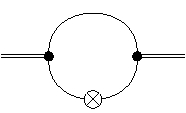
\includegraphics[width=\textwidth]{figs/TikZ/fermion_contribution}
% 	\subcaption{Fermions.}
% \end{subfigure}
% \hfill
% \begin{subfigure}{0.3\textwidth} 
% 	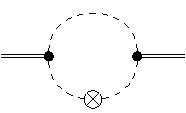
\includegraphics[width=\textwidth]{figs/TikZ/scalar_contribution}
% 	\subcaption{Scalars.}
% \end{subfigure} 
% \hfill
% \begin{subfigure}{0.3\textwidth} 
% 	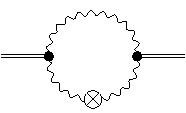
\includegraphics[width=\textwidth]{figs/TikZ/gauge_field_contribution}
% 	\subcaption{Gauge Fields.}
% \end{subfigure} 
% \hfill
% \caption{Different matter contributions to the graviton anomalous dimension $\eta_h$.}	
% \end{figure}
 

 
%  \begin{figure}[t]
% \centering
% \hfill
% \begin{subfigure}{0.3\textwidth} 
%	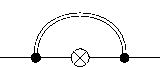
\includegraphics[width=\textwidth]{figs/TikZ/graviton_fluctuations1}
% \end{subfigure}
% \hfill
% \begin{subfigure}{0.3\textwidth}
% \vspace{-3.5pt}
% 	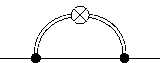
\includegraphics[width=\textwidth]{figs/TikZ/graviton_fluctuations2}
% \end{subfigure} 
% \hfill
% \begin{subfigure}{0.3\textwidth} 
% 	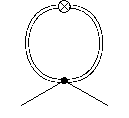
\includegraphics[scale = 1.5]{figs/TikZ/graviton_fluctuations3}
% \end{subfigure} 
% \hfill
% \caption[Contributing diagrams to the fermion anomalous dimension $\eta_D$.]{Contributing diagrams to the fermion anomalous dimension $\eta_D$. Analogous contributions arise for external scalars and gauge fields to $\eta_S$ and $\eta_V$.} 	
% \end{figure}
 
 